\part{Desenvolvimento}

\chapter[Fundamentação Teórica]{Fundamentação Teórica}

Este capitulo descreve os principais conceitos abordados neste trabalho,
 descrevendo a diferença entre linguagens compiladas e linguagens interpretadas,
 o modelo de execução \textit{just in time}, máquinas virtuais,
 o processo de compilação e sobre os métodos aqui trabalhados.
 
\section{Linguagens compiladas e linguagem interpretadas}

Uma linguagem de programação é um método padronizado que possui
 um conjunto de instruções para comunicação entre o homem
 e o computador \cite{ref1}, através de um conjunto de regras
 definidas tanto sintaticamente quanto sematicamente \cite{ref2}.
 Com uma linguagem
 de programação é possível especificar precisamente um conjunto de regras
 sobre  as quais dados serão armazenados ou transmitidos e criar algoritmos
 que representam operações ou resolvam problemas.
    
Para que um algoritmo escrito em uma linguagem de programação seja executado 
por um computador é necessário a criação de um arquivo de texto contendo um 
conjunto de palavras ou símbolos escritos de forma ordenada  e de maneira 
lógica \cite[pág. 3]{ref3}. Este arquivo é chamado de código fonte.
    
Antes da execução, a linguagem de programação escrita no código fonte deve
 ser convertida (através do processo de compilação), traduzida (através do 
processo de interpretação) ou convertida e traduzida (forma hibrida) em um 
código de máquina \cite[pág. 2]{ref4}.

\subsection{Compilação}
\label{Compilação}

No processo de compilação a linguagem de programação contida no código fonte
 deve ser transformada em uma linguagem de máquina, a qual será posteriormente
 executada pelo processador \cite{ref2}. 

O processo de compilação requer a utilização de um compilador, o qual consiste
 em um programa ou conjunto de programas  que tem como entrada o código fonte 
escrito em uma linguagem de programação e como saída, cria um programa sematicamente 
equivalente uma outra linguagem, chamado de código objeto \cite[pág. 2]{ref4}.

Após a compilação, a execução do código objeto criado a partir do
 código fonte de entrada deve ser requisitado pelo usuário para que o processador 
execute as instruções de máquina \cite[pág. 17]{ref6}.

As linguagens que, em geral, são compiladas, tem melhor performance em relação
 as linguagens que, em geral, são interpretadas. Isso porque as decisões que são
 tomadas em tempo de compilação não são necessárias no tempo de execução \cite[pág. 2]{ref3}.
Por exemplo, se um compilador garantir que em uma variável \texttt{x} seja sempre alocada 
em uma mesma posição na memória,  ele pode gerar instruções de máquina que 
acesse esta localização sempre que se referenciar a variável \texttt{x}. 
Por outro lado, um interpretador precisa procurar por \texttt{x} em uma tabela a cada 
acesso, a fim de determinar sua localização \cite[pág. 167]{ref2}.

Como exemplos de linguagens que, em geral, são compilada, temos Ada, ALGOL, 
BASIC, C, C++, COBOL, Cobra, Common Lisp, D, Delphi, Eiffel, Fortran, 
Objective-C, Pascal, Visual Basic, Visual Prolog.

\subsection{Interpretação}

No processo de interpretação, o código fonte é passado para um programa chamado
 interpretador, o qual é responsável pela leitura do código e pela tradução, 
em tempo real, deste código em instruções a serem executadas pelo sistema 
operacional ou  pelo processador \cite{ref2}. No caso de linguagens que são, em geral, 
interpretadas, costuma-se nomear os códigos-fonte como scripts, embora esta não seja 
uma regra geral.

Ao contrário do compilador, o interpretador faz a leitura do código fonte e 
executa  as respectivas instruções em tempo real. Isso faz com que  códigos 
interpretados tenham maior flexibilidade e um melhor diagnóstico (exibição de 
mensagens de erros) do que  códigos compilados. A interpretação também pode lidar 
melhor com linguagens de programação nas quais características fundamentais, 
tais como  o tamanho e  o tipo das variáveis, podem depender dos dados de 
entrada \cite[pág. 17]{ref6}.

Mesmo que uma linguagem seja projetada inicialmente para ser compilada é possível que exista 
interpretadores para estas linguagens, como é o caso do CINT\footnote{
Interpretador de código C/C++ encontrado em \url{https://root.cern.ch/cint}.}
 e CLING\footnote{Interpretador de código C/C++ com back-end clang encontrado em
  \url{https://root.cern.ch/cling}.}.Estes interpretadores podem ajudar no 
  processo de desenvolvimento como descrito acima, no entanto existem 
  limitações, como no caso do CINT\footnote{
  \url{https://root.cern.ch/viewvc/branches/v5-34-00-patches/cint/doc/limitati.txt }}:

\begin{itemize}
	\item não é possível definir um novo tipo de dado baseado em estrutura(\textit{struct}) dentro de uma função;
    \item não suporta o tipo \textit{unsigned long long}, interpretando-o como long long;
    \item o próprio \textbf{CINT} contém a definição do tipo bool, e carrega o mesmo na execução do programa;
    \item na declaração de ponteiro é necessário um espaço em branco antes e depois do '*'; 
    \item não aceita o operador de sequenciamento ‘,’; 
    \item um dos maiores problemas do \textbf{CINT} é a definição de macros:
 ele suporta apenas macros simples.
\end{itemize}

Sem  o recurso da interpretação, seria uma tarefa deveras complexa implementar 
alguns recursos  presentes em linguagens Lisp e Prolog onde, por exemplo, 
um programa pode escrever novas peças de si mesmo e executá-las em tempo real
 \cite[pág. 17]{ref6}.
Como exemplos de linguagens que, em geral, são interpretadas, temos ActionScript,
 APL, ASP, BASIC, C\#, CYBOL, Java, JavaScript, Lisp, Logo, Lua, PHP, Python, Ruby,
 Scheme, Smalltalk, VBScript.
 

\subsection{Máquinas Virtuais}

Para algumas linguagens existe o caso em que o compilador tem o papel
 de converter o código fonte em um \textit{byte code} \cite[pág. 49]{ref9}. 
O \textit{byte code}
é uma linguagem de baixo nível  similar a linguagem de máquina, que 
deve ser interpretada por um outro programa chamado Maquina Virtual (\textit{Virtual Machine -- VM}).

Esta estratégia mista de pré-compilar o código para uma linguagem 
intermediária e interpretá-la em uma máquina virtual é denominada 
estratégia híbrida. 

Como exemplo de linguagens que utilizam, em geral, a estratégia híbrida, temos 
 Java, Python, JRuby, Oxygene, Rhino, Nashorn, JGNAT, Jython, Rakudo Perl 6.

\subsection{Just In Time}

O termo \textit{Just In Time} -- JIT -- veio de um novo modelo de  negócio da
 indústria manufatureira: uma estratégia onde a produção 
ou compra era feita sobre demanda, ao invés da utilização de estoques
 \cite[pág. 177]{ref10}. 
Este modelo tem como vantagens menores custos com armazenamento, 
menos desperdícios, resposta mais rápida aos clientes e maior 
produção potencial.

Na compilação, esta analogia se adapta bem por que um compilador JIT 
não armazena os binários do programa no disco (o estoque), mas começa 
a compilação apenas de partes do programa necessárias durante a execução
 \cite[pág. 8]{ref2}.

Foram desenvolvidas, principalmente para linguagens que são, em geral, 
interpretadas, ferramentas que se valem do JIT para acelerar a interpretação
 e execução dos códigos-fonte (scripts) como, 
por exemplo, o PyPy para a linguagem Python.\footnote{\url{http://pypy.org/}}


\section{Compilação}

\subsection{Preprocessadores}


Antes de um código-fonte passar pelo processo de compilação, pode ser
 necessária a execução de um programa, denominado preprocessador, que
 tem como responsabilidade preparar o código-fonte para a compilação. 

Dentre as possíveis tarefas e características comuns a um preprocessador,
 podemos citar:

\begin{itemize}

\item \textit{Processamento de macros}: um preprocessador pode permitir que um usuário 
    defina macros que sejam abreviações para construções mais longas \cite[pág. 8]{ref3};

\item \textit{Inclusão de arquivos}: um preprocessador pode incluir arquivos cabeçalho no
     texto do programa. Por exemplo, o preprocessador faz com que o conteúdo de
     um arquivo externo seja transcrito no código-fonte no ponto onde existe a 
    marcação para sua inclusão \cite[pág. 8]{ref2};

\item \textit{Preprocessadores “racionais”}: este tipo de preprocessador é responsável 
    por permitir a construção de macros utilizando condicionais \textit{while} ou \textit{if} mesmo
     em linguagens que não suportem tais estruturas \cite[pág. 8]{ref2};

\item \textit{Extensões de linguagens}: são formas de conferir maior poder as linguagens
     através de macros embutidas. Por exemplo, 
    Equel\footnote{\url{http://www.eecs.berkeley.edu/~wong/wong\_pubs/wong46.pdf}. Acessado em 11 de junho de 2015.} é uma linguagem de 
    interrogação embutida em C que permite a manipulação de banco de dados. 
    Os enunciados começados com \texttt{\#\#} são considerados pelo preprocessador como
     comandos de acesso ao banco de dados, os quais não fazem parte da 
    linguagem C e, quando traduzidos, são convertidos em rotinas que tratam 
    este acesso ao banco de dados \cite[pág. 8]{ref3}.

\end{itemize}

\subsection{Compilação}

No processo de compilação tradicional, o compilador atua em duas fases 
principais: análise e síntese \cite[pág. 26]{ref6}. A Figura \ref{fig01}
 ilustra estas fases. 

\begin{figure}[h]
    \centering
        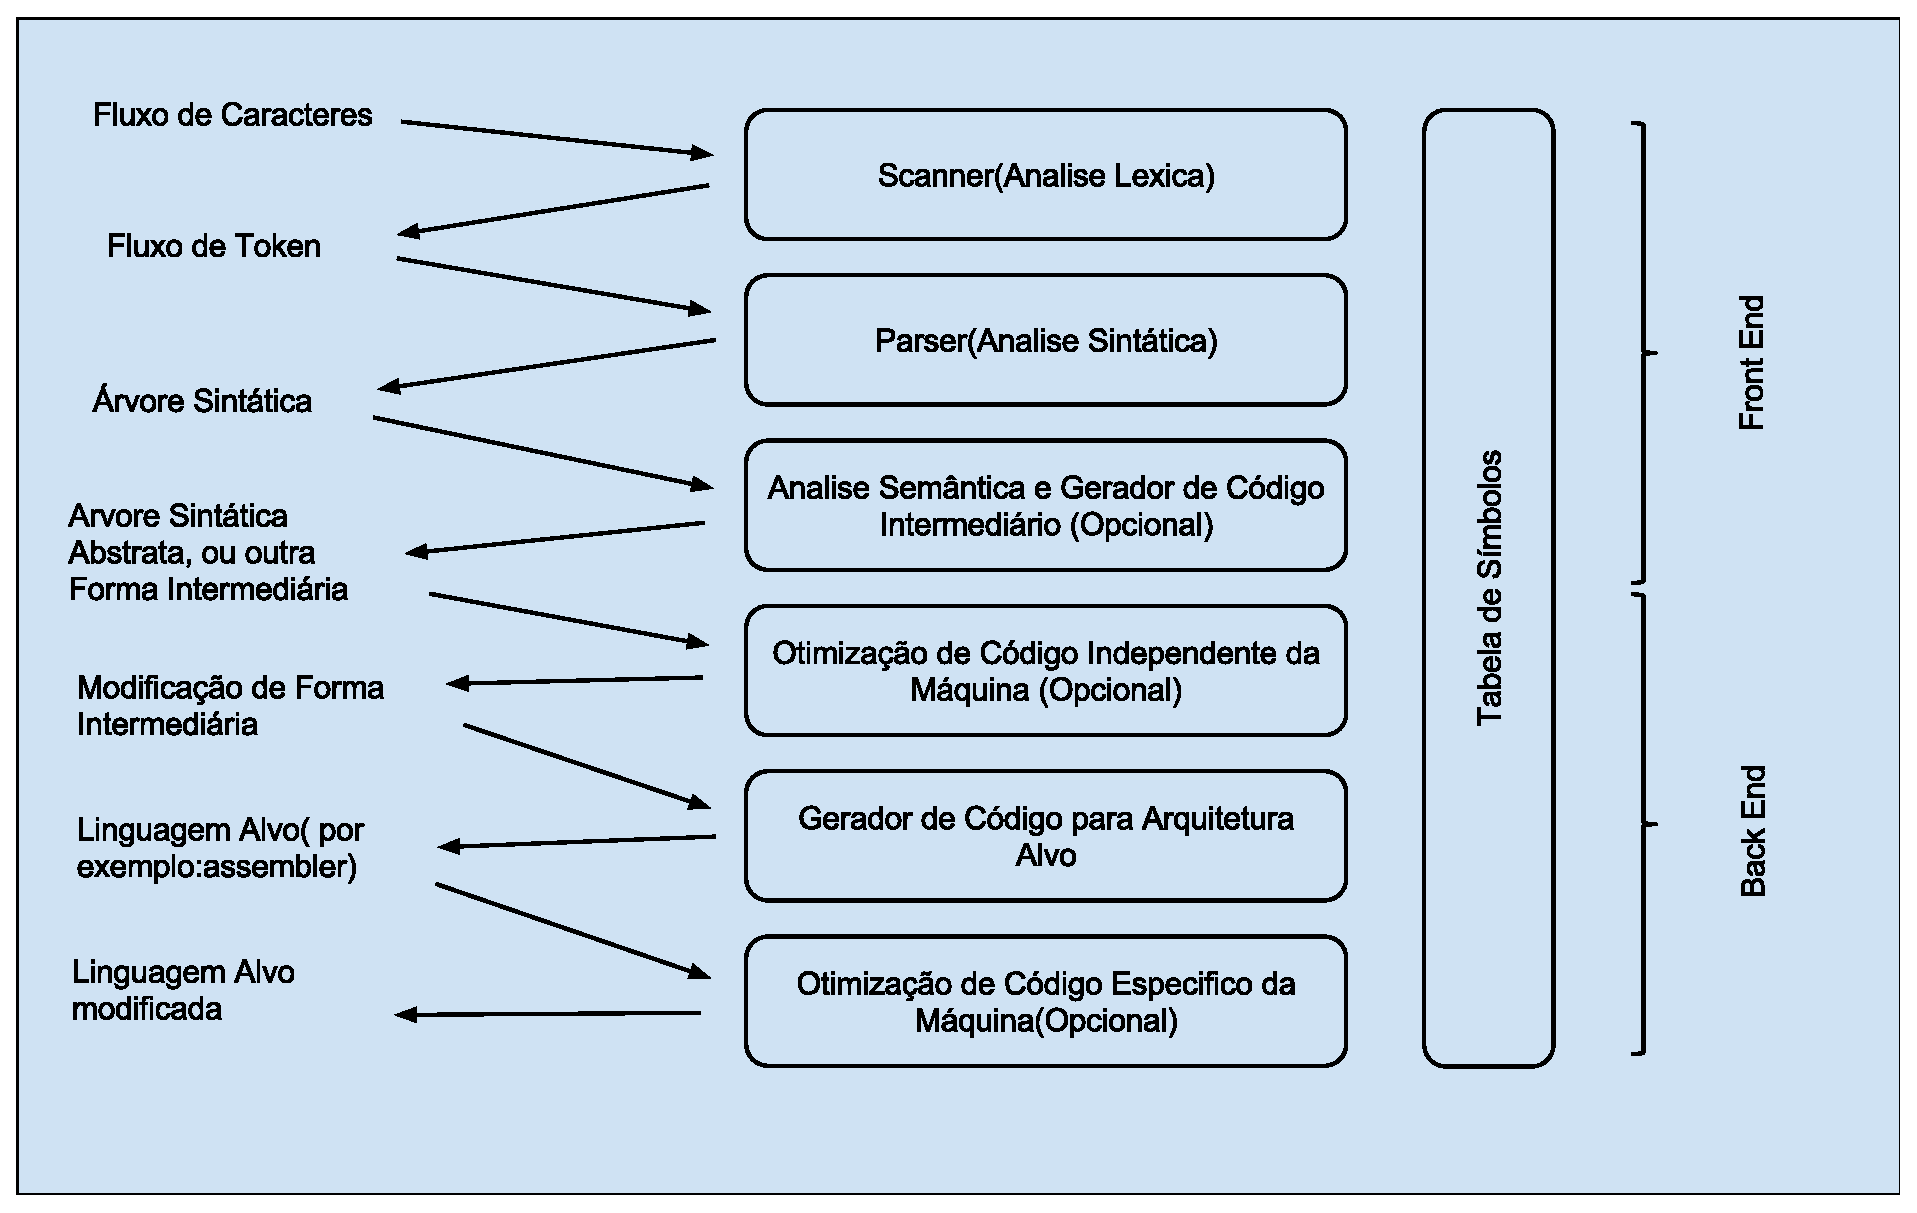
\includegraphics[keepaspectratio=true,scale=0.45]{figuras/fases_da_compilacao.eps}
    \caption{Fases da Compilação \cite[pág. 26]{ref6}, com adaptações.}
    \label{fig01}
\end{figure}

A fase de análise (ou \textit{front-end}) de um compilador é a fase que 
tem como objetivo entender o código fonte e  representá-lo em uma 
estrutura intermediária que facilite sua manipulação posterior. 
Esta fase é subdividida em análise léxica, análise sintática, 
análise semântica e geração de código intermediário \cite[pág. 36]{ref6}.

A fase de síntese (ou \textit{back-end}) de um compilador é a fase que tem 
como objetivo realizar a geração de código final, otimizando o código 
analisado na fase de sintase e gerando um código sematicamente igual ao 
código fonte e com melhorias de performance e espaço. Esta fase é 
subdividida em otimização de código independente do alvo, geração de 
código alvo e otimização de código para o alvo específico \cite[pág. 36]{ref6}.

\subsection{Análise Léxica}
    
A análise léxica é a primeira fase a ser executada pelo compilador \cite[pág. 59]{ref15}. 
A função do analisador léxico, também denominado \textit{scanner}, é ler o código fonte, 
caractere a caractere, buscando a separação e  a identificação dos elementos do 
programa, denominados símbolos léxicos ou tokens \cite[pág. 195]{ref16}. Assim, é 
produzida uma sequência de tokens que será utilizada na análise sintática \cite[pág. 38]{ref3}. 

Esta fase também tem a importância de realizar a remoção de elementos 
“decorativos” do programa, tais como espaços, tabulações, caracteres de 
avanço e comentários \cite[pág. 59]{ref15}. Para auxiliar a construção deste analisador,
 estão disponíveis uma série de geradores automáticos de analisadores léxicos, 
cujo objetivo é reduzir o esforço de programação deste tipo de ferramenta, 
especificando-se apenas os tokens a serem reconhecidos \cite[pág. 50]{ref18}.

\subsection{Análise Sintática}

A análise sintática, ou análise gramatical, é o processo de determinar 
se uma cadeia de símbolos léxicos pode ser gerada por uma gramática pré-definida
 \cite{ref19}. O analisador sintático é o responsável por verificar se os 
símbolos contidos no código fonte formam um programa válido ou não \cite[pág. 38]{ref20}.

A maioria dos métodos de análise sintática são de dois tipos, denominados 
\textit{top-down} ou \textit{bottom-up} \cite[pág.  227]{ref21}. Como indicado por 
seus nomes, os analisadores sintáticos \textit{top-down} constroem árvores 
do topo para as folhas, enquanto o analisadores \textit{bottom-up} começam das 
folhas e constroem a árvore de baixo para cima até chegar na raiz. Em ambos os
 casos são percorridas da esquerda para a direita, 
símbolo a símbolo. Estes dois tipos são utilizados devido seu potencial 
expressivo para descrever a maioria das construções sintáticas das linguagens 
de programação \cite[pág. 38]{ref20}. Para auxiliar na criação de analisadores sintáticos 
existem disponíveis uma série de geradores automáticos, como por exemplo, 
o \textit{Flex}\footnote{\url{http://dinosaur.compilertools.net/}. Acessado no dia 20/06/2015.}, 
o \textit{Bison}\footnote{\url{http://www.gnu.org/software/bison/} Acessado no dia 20/06/2015.}
 e o \textit{JavaCC}\footnote{\url{https://javacc.java.net/}. Acessado no dia 20/06/2015.}
 \cite[pág. 30]{ref22}.

\subsection{Análise Semântica}

O analisador semântico tem como função prover métodos para que as estruturas 
construídas pelo analisador sintático possam ser avaliadas ou executadas \cite[pág. 337]{ref23}. 
Estas validações são feitas para assegurar que certos tipos de erros de 
programação sejam detectados e reportados. Os  exemplos de verificação incluem 
declaração de tipo, declaração de funções, sobrecarga de funções, sobrecarga de 
operadores, verificação de fluxo de controle, verificação de operações lógicas e 
aritméticas válidas entre variáveis e a verificação de unicidade de variáveis em 
determinados escopos da linguagem \cite[pág. 147]{ref6}.

\subsection{Gerador de Código Intermediário}

Após produzir uma árvore sintática sematicamente correta, o compilador é capaz de
 produzir uma linguagem de representação intermediária do código fonte. Uma linguagem 
intermediária está mais próxima de uma linguagem de objeto do que da linguagem do código fonte. 
No entanto, a linguagem  intermediária permite uma manipulação mais fácil do que o 
código de máquina ou o \textit{Assembly} \cite[pág. 8]{ref25}. 

Um tipo bem conhecido de linguagem intermediara é o código (ou sentença) de três 
endereços \cite[pág. 247]{ref26}. Este código é uma sequência de enunciados na forma geral, apresentada 
 no Código \ref{codigo01},

\begin{lstlisting}[language=C++,caption={Código de três endereços},
											label=codigo01]
   x:=y op z
\end{lstlisting}
onde \texttt{x}, \texttt{y}, \texttt{z} são nomes, constantes ou objetos de dados 
temporários criados pelo compilador e \texttt{op} representa um operador qualquer,
 tal como um operador de ponto fixo, flutuante ou um operador lógico sobre dados
 booleanos \cite[pág. 201]{ref6}. Uma forma prática de representar sentenças de três endereços é o uso
 de quádrupla (operador, argumento 1, argumento 2 e resultado). 
Este esquema de representação de código intermediário é o preferido por diversos
 compiladores, principalmente por aqueles que executam extensivas otimizações de
 código, uma vez que o código intermediário pode ser manipulado mais 
facilmente \cite[pág. 604]{ref5}. Além destas representações existem outras como as 
árvores, grafos acíclicos dirigidos (DAG) e a notação polonesa \cite[pág. 96]{ref29}.

Para garantir que um código tenha o seu desempenho ampliado e utilize menos 
espaço em disco, a fase de otimização de código busca examinar 
estrategicamente o código intermediário produzido na fase anterior e, com o 
uso de técnicas de otimização, produzir um código mais eficiente \cite[pág. 796]{ref30}
. A otimização de código pode ocorrer em duas etapas: uma após a geração de 
código intermediário e a outra depois da geração do código para a máquina 
alvo \cite[pág. 34]{ref6}. 
Para a execução desta etapa são utilizadas técnicas para detectar 
padrões dentro de um código produzido e substituí-los por códigos mais
 eficientes \cite[pág. 604]{ref5}. Entre as técnicas usadas realizadas estão a 
substituição de expressões que podem ser calculadas durante o tempo 
de compilação, movimentação de código, eliminação de sub-expressões 
redundantes, desmembramento de laços, eliminação de variáveis de indução, 
substituição de multiplicação pelo \textit{shift} binário, redução da 
quantidade de laços, entre outras \cite[pág. 796]{ref30}.

\subsection{Geração de Código}

Gerador de código é a parte ou componente do compilador responsável por 
realizar o mapeamento da linguagem intermediária otimizada para a linguagem 
alvo. Caso a linguagem alvo seja um código de máquina,  registradores ou 
localização de memoria são selecionados para armazenar valores das 
variáveis usadas no programa. Então, o código intermediário é traduzido em 
sequência para instruções de máquina que realizarão as operações \cite[pág. 10]{ref3}.
Mesmo que o código traduzido seja otimizado, após a tradução para a 
linguagem alvo é  possível que novas otimizações sejam feitas, como
 a otimização específica apresentada no Código \ref{otimizacao}.


\begin{lstlisting}[language=C++, caption={Exemplos de otimização específica},
                                                              label=otimizacao]
Propagacao de constante

r2 := 4                r2 := 4                  r3 := r1 + 4
r3 := r1 + r2   vira   r3 := r1 + 4  e entao    r2 := ...
r2 := ...              r2 := ...

Duplicacao de Constantes

r2 := 3 x 2 vira r2 := 6

Eliminacao de Atribuicao e uso de variavel

r2 := r1 + 5              r2 := r1 + 5
i  := r2           vira   i   := r2
r3 := i                   r3 := r2 x 3
r3 := r3 x 3
\end{lstlisting}


\subsection{Assembly}

Segundo Michael L. Scott, um código de máquina é uma sequência de \textit{bits} que
 corresponde a uma instrução executada por um processador, realizando 
operações de adições, comparações, movimento de informação de uma localização
 da memória, entre outros. Detalhar instruções de máquina a nível de \textit{bits} é 
uma tarefa trabalhosa \cite[pág. 5]{ref6}. 

Um programa capaz de realizar o cálculo do máximo divisor comum através do 
algoritmo de Euclides estendido pode ser representado  em código de máquina 
usando notação hexadecimal para a representação dos \textit{bits}, conforme apresentado
 no Código \ref{codigo_02} \cite[pág. 5]{ref6}.


\begin{lstlisting}[language=Pascal, caption={Algoritmo de 
									   Euclides Estendido, com adaptações},
                                                            label=codigo_02]
 55 89 e5 53  83 ec 04 83  e4 f0 e8 31  00 00 00 89  c3 e8 a2 00
 00 00 39 c3  74 10 8d b6  00 00 00 00  39 c3 7e 13  29 c3 39 c3
 75 f6 89 c1  24 e8 6e 00  00 00 8b 5d  fc c9 c3 29  d8 eb eb 90
\end{lstlisting}

Para facilitar a comunicação entre uma linguagem composta apenas por \textit{bits} e 
uma linguagem entendida por um desenvolvedor foi necessário a criação de uma
 linguagem que permitisse que as operações em \textit{bits} fossem representadas por 
abreviações ou símbolos que facilitassem o entendimento por parte do programador.
 Assembly é a linguagem escolhida para estas representações, onde cada 
instrução do processador foi mapeada em um mnemônico, representados geralmente 
por acrônimos do inglês (por exemplo, \texttt{mov} representa ‘mover’, \texttt{rep} 
representa repetição e assim por diante) \cite[pág. 5]{ref6}.

O mesmo programa mostrado no Código \ref{codigo_02} pode ser representado 
em assembly, conforme ilustrado no Código \ref{codigo_03} \cite[pág. 5]{ref6}. 

\begin{lstlisting}[language=Pascal,caption={Algoritmo de 
                                 Euclides estendido em Assembly , com adaptações},
                                                            label=codigo_03]
    pushl %ebp              jle   D
    mov   %esp, %ebp        subl  %eax, %ebx
    pushl %ebx           B: cmpl  %eax, %ebx   
    subl  $4, %esp          jne   A
    andl  $-16, %esp     C: call  %ebx, (%esp)
    call  getint            call  putint
    movl  %eax, %ebx        movl  -4(%ebp), %ebx
    call  getint            leave
    cmpl  %eax, %ebx        ret
    je    C              D: subl  %eax, %eax
 A: cmpl  %eax, %ebx        jmp   B

\end{lstlisting}

Para converter um programa de assembly para um código de máquina é necessário
 um montador, denominado Assembler. O montador é um programa que realiza a 
parametrização das instruções da linguagem Assembly para os \textit{bits} 
correspondentes da linguagem de máquina (também chamado de \textit{opcode}) \cite[pág. 6]{ref6}.

\subsection{Linking}


\begin{figure}[h]
    \centering
        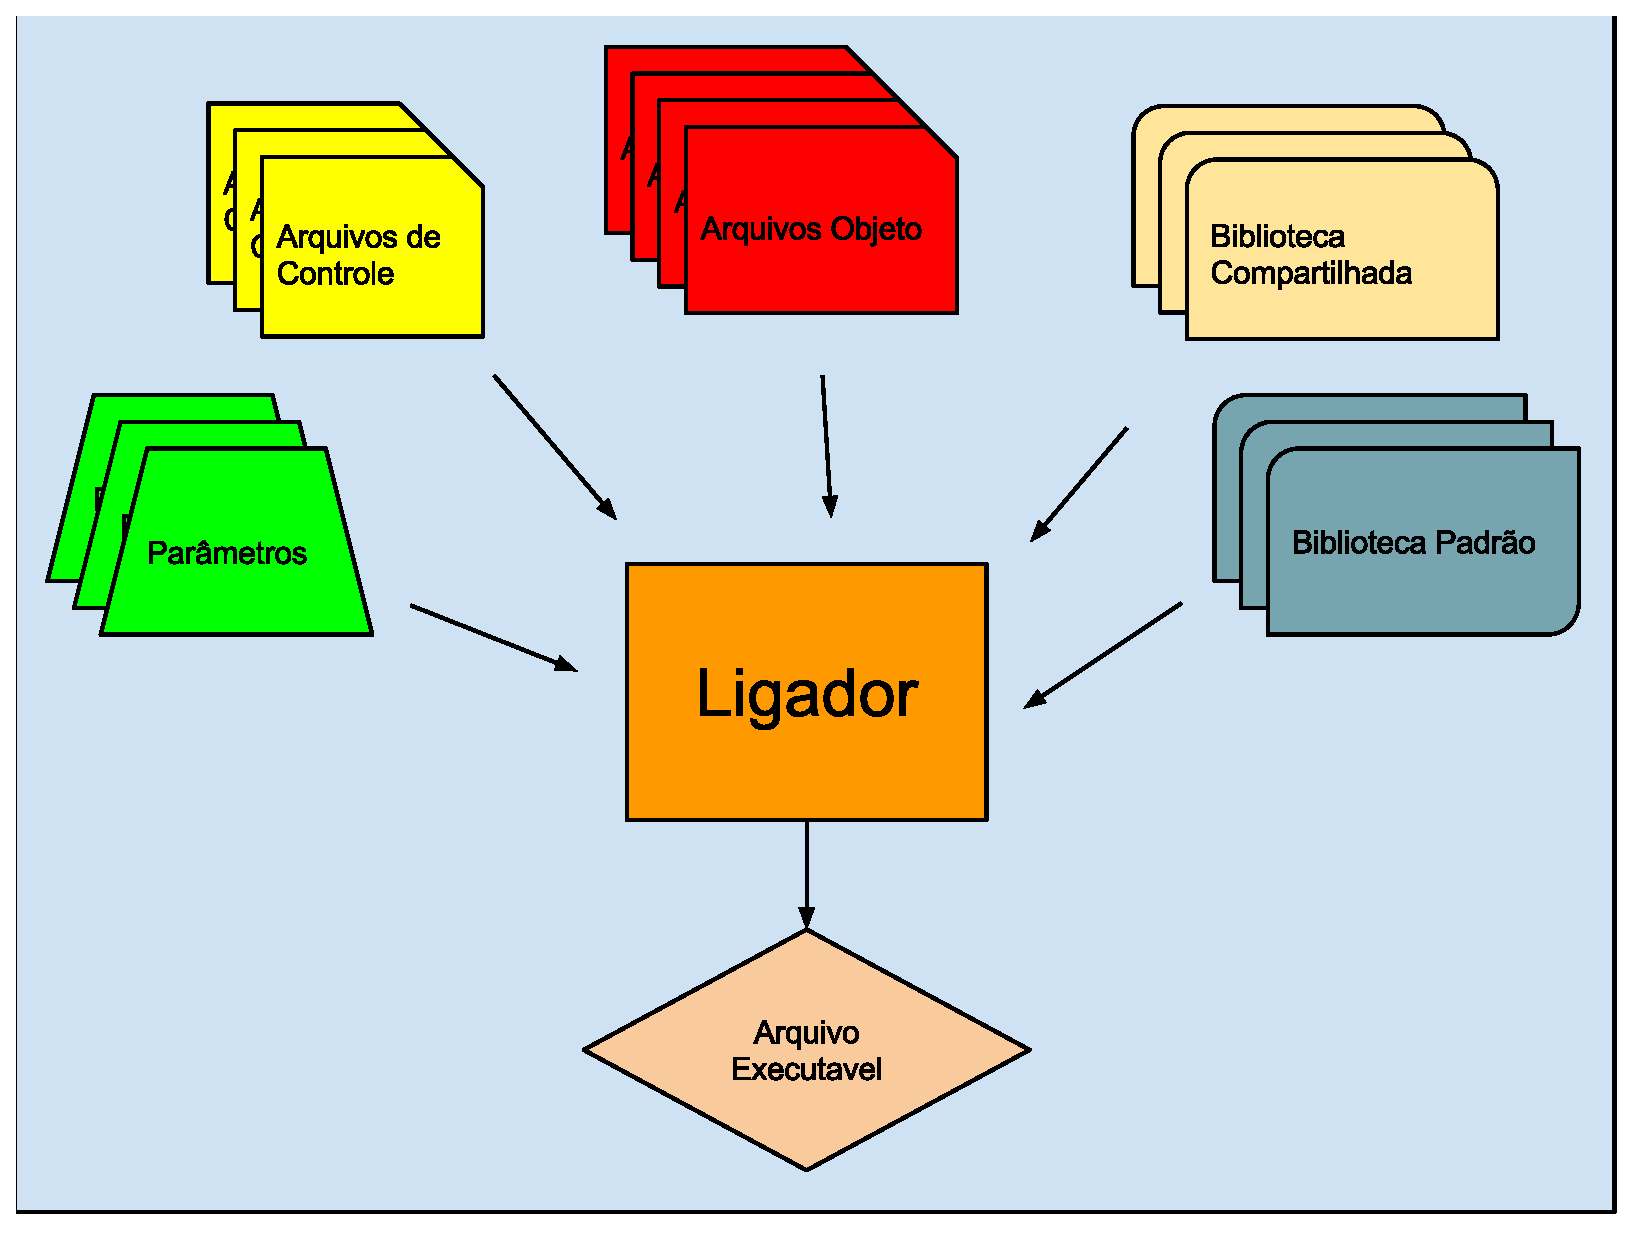
\includegraphics[keepaspectratio=true,scale=0.5]{figuras/ligador.eps}
    \caption{Ligação entre objetos \cite[pág.  7]{ref36}, com adaptações.}
    \label{fig03}
\end{figure}

Um compilador é capaz de realizar a compilação de partes de programas e gerar
 objetos que podem ser combinados para formar um programa executável. 
\textit{Linker} (ou Ligador) é um programa capaz de realizar a junção 
de objetos gerados por um compilador, ligando nomes abstratos em nomes
 mais concretos, permitindo o desenvolvedor escrever códigos usando nomes 
mais próximos da sua realizade \cite{ref36}.


 Basicamente o Linker liga um nome ou símbolo escrito por um desenvolvedor e
 referencia a localização do inicio do código que possui a função ou o dado
 estático. Como no exemplo descrito por John Levine, o linker pega um 
referência escrita como \texttt{getline}  e vincula a “uma localização de 612 \textit{bytes}
no inicio de um código executável do módulo \texttt{iosys}” \cite[pág. 7]{ref36}. 

A fase de link-edição tem dois passos. No primeiro o Linker recebe como 
entrada um conjunto de arquivos objetos, bibliotecas e parâmetros e produz
 como resultado um arquivo de saída, como mostrado na Figura \ref{fig03}
 \cite[pág. 13]{ref36}. Neste passo é criada uma tabela com 
todos os segmentos definidos nos arquivos fontes e uma tabela de símbolos 
importados ou exportados. Depois o Linker atribui uma localização numérica 
para cada símbolo, determinando o tamanho e a localização dos segmentos no
 espaço de endereço final. O segundo passo usa as informações do primeiro
 para controlar a link-edição, ajustando os endereços de memória do código e
 escrevendo os endereços de código realocado no arquivo de saída
 (programa executável).


\subsection{Bibliotecas}

Após algum tempo utilizando compiladores e linkers, muitos 
desenvolvedores perceberam que poderiam economizar tempo e esforço 
reutilizando pedaços de códigos escritos em outros programas. Para evitar a
 cópia de arquivos entre projetos surgiram as chamadas bibliotecas \cite[pág.  227]{ref36}.

Biblioteca é um conjunto de códigos compilados que podem ser incorporados a
 um ou mais de um projetos, como mostrado nas Figura \ref{fig04}, e Figura
 \ref{fig05}. A organização de códigos em bibliotecas permite que 
programas sejam mais modulares, mais rápidos de recompilar e mais 
fáceis de manter \cite{Lasca}.

As bibliotecas podem ser divididas em três tipos: estáticas, 
dinâmicas e compartilhadas \cite{Lasca}.

\begin{figure}[h]
    \centering
        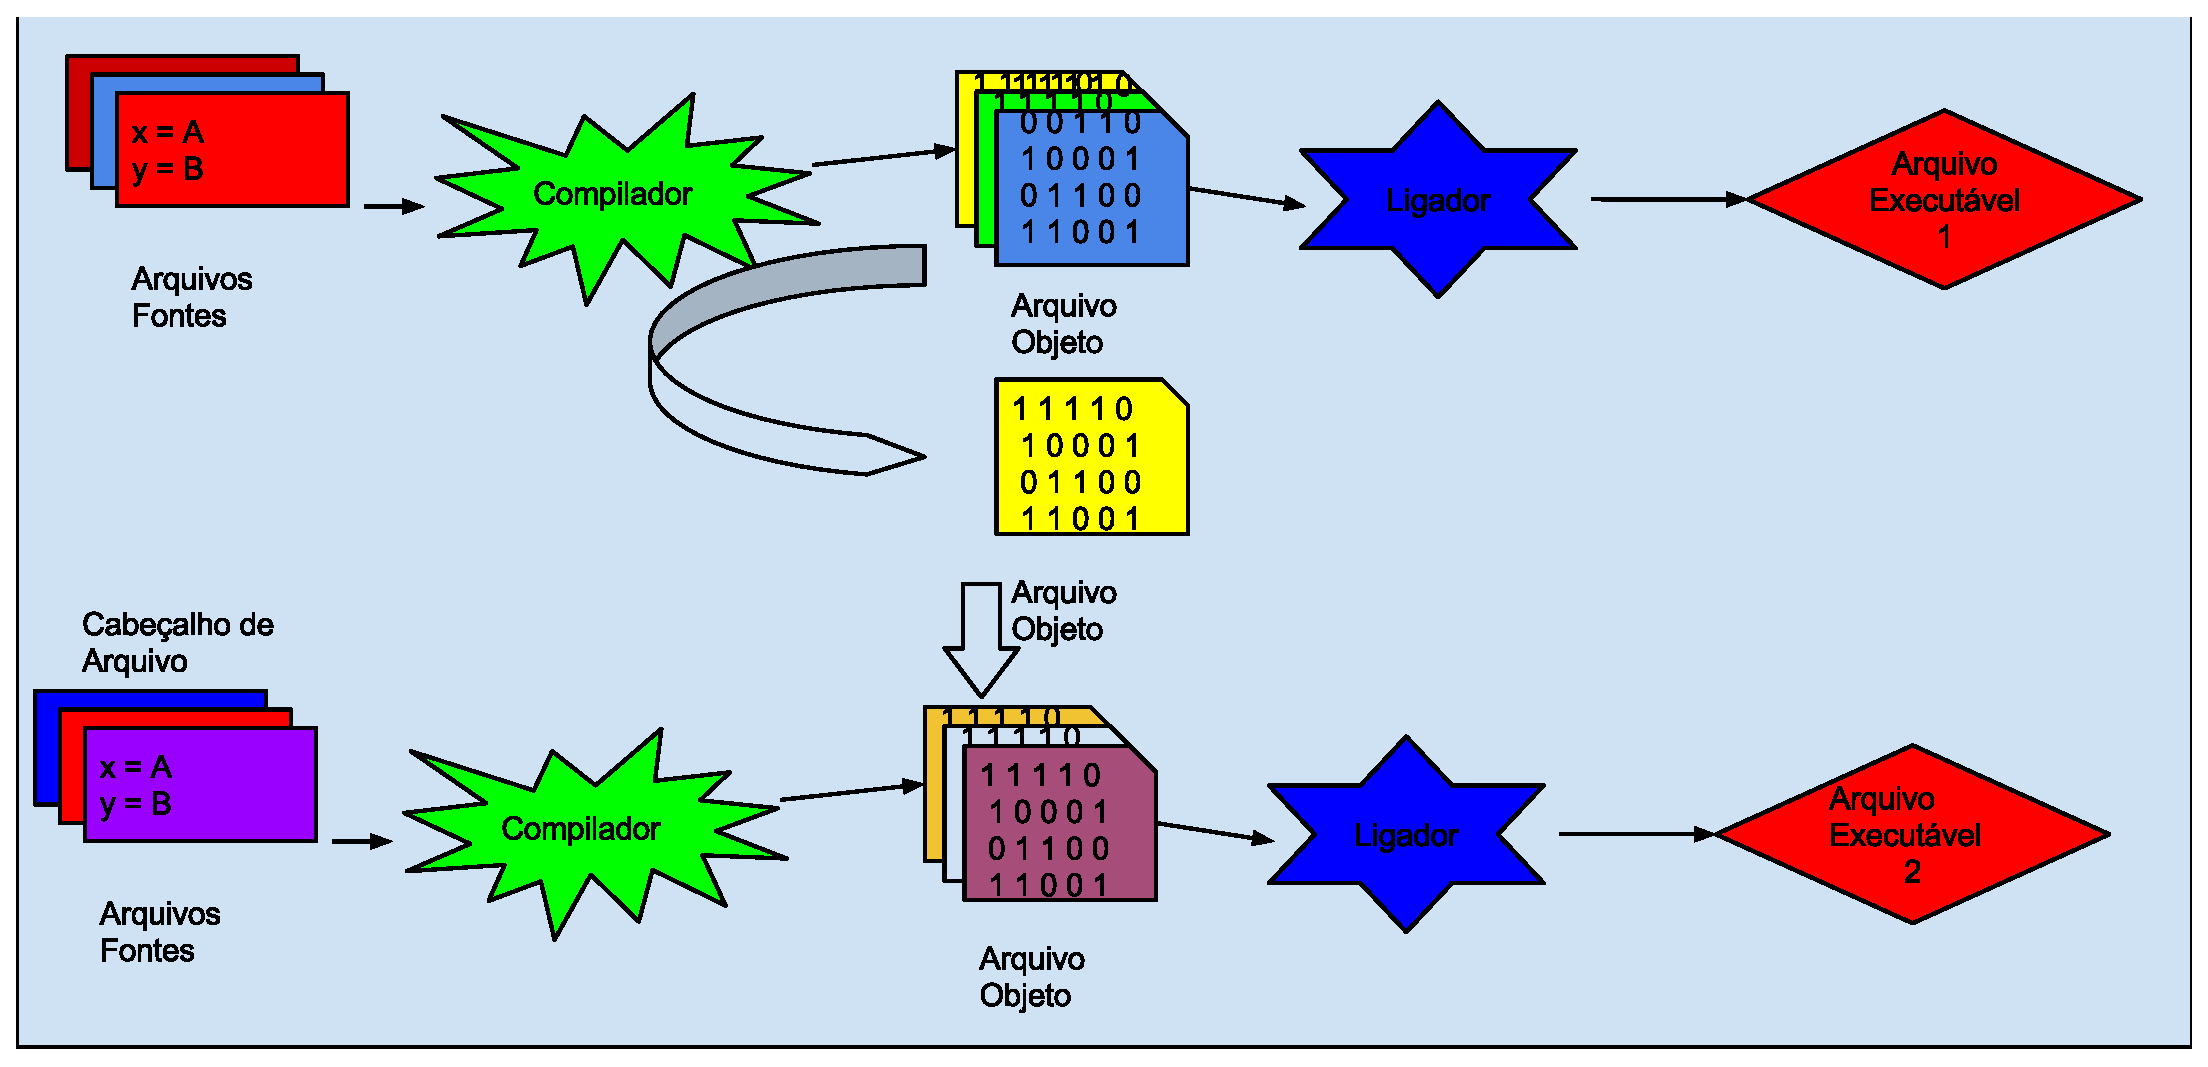
\includegraphics[keepaspectratio=true,scale=0.38]{figuras/reuso_lib_estatica.eps}
    \caption{Reuso com biblioteca estática \cite[pág.  54]{ref39}, com adaptações.}
    \label{fig04}
\end{figure}

\begin{figure}[h]
    \centering
        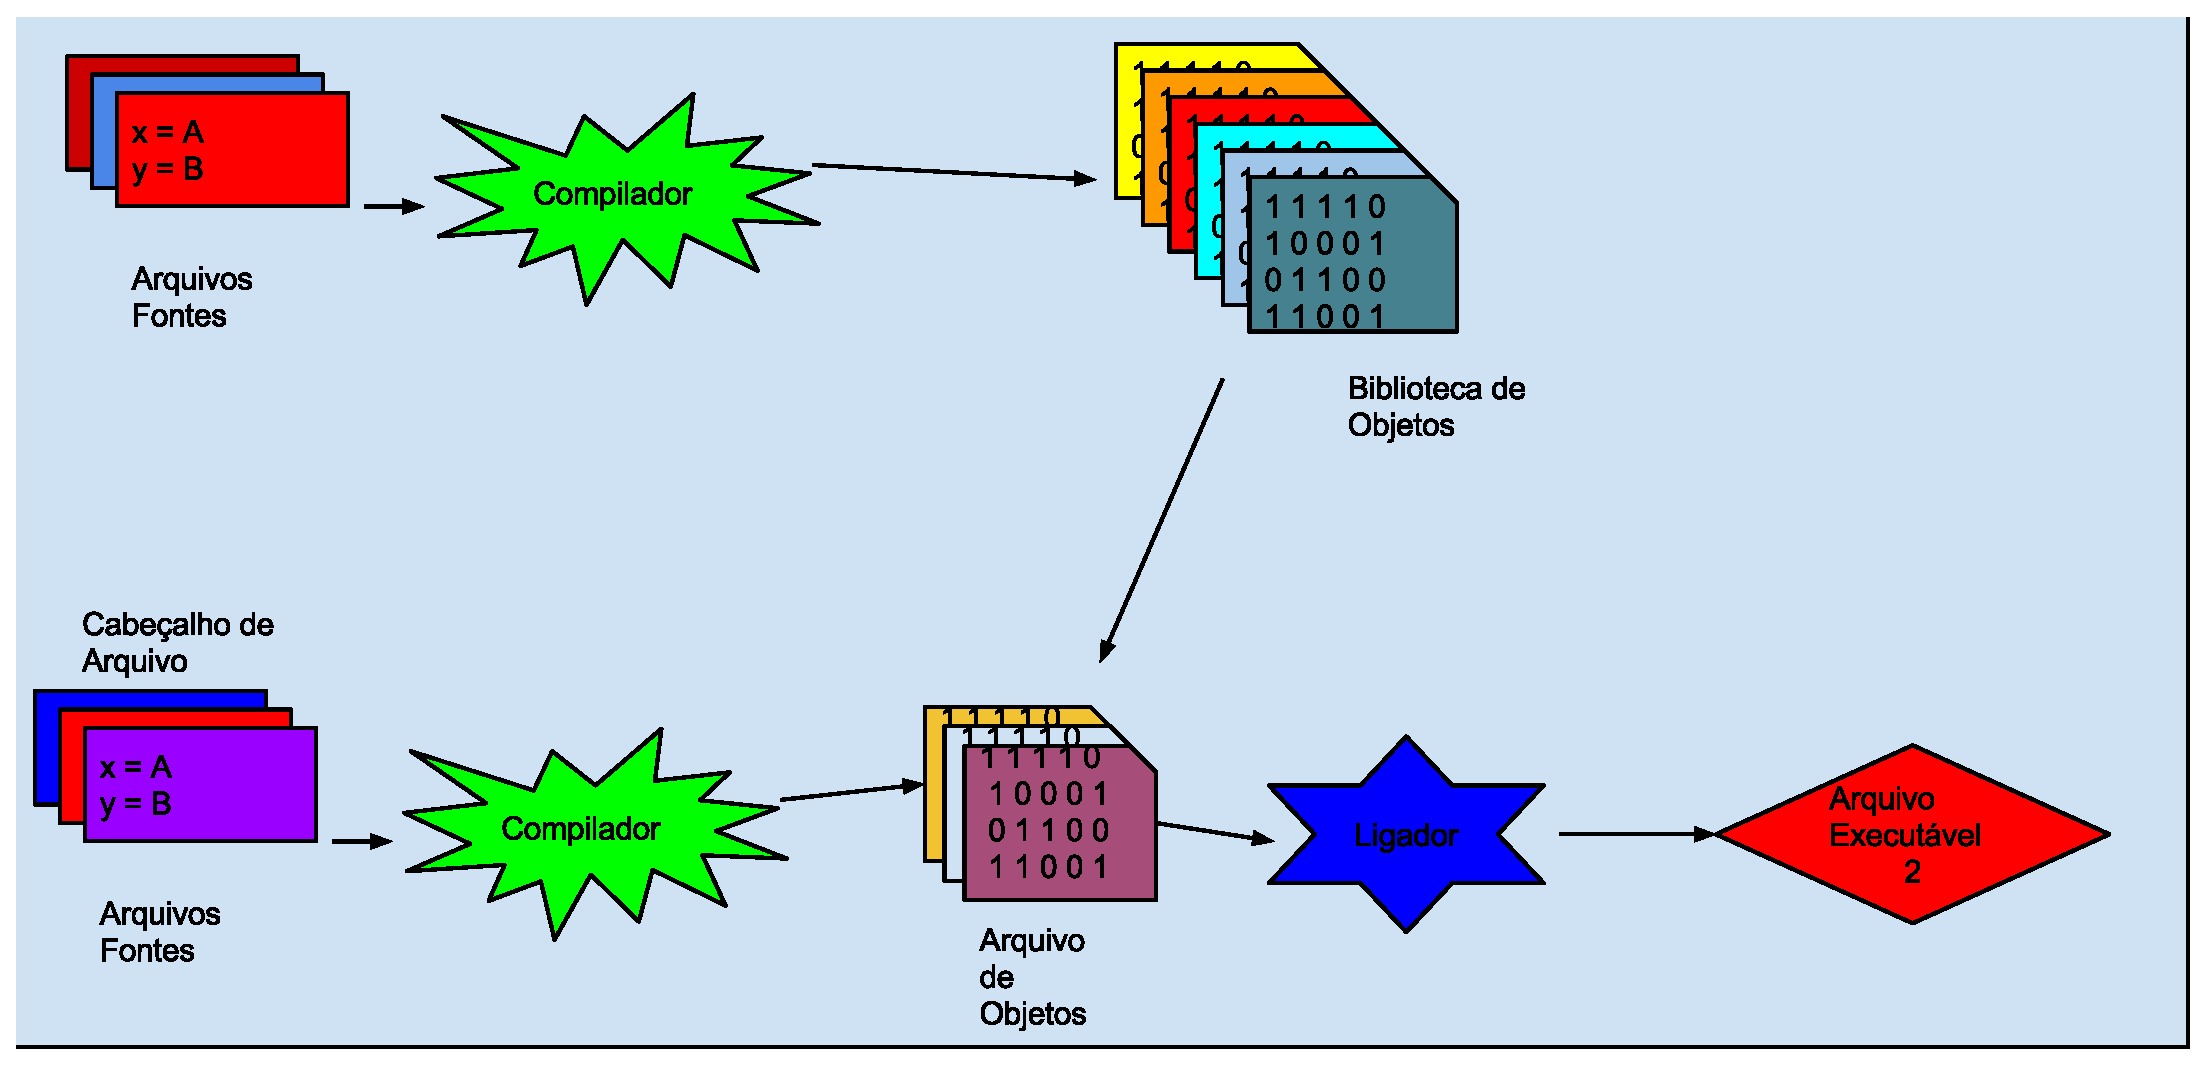
\includegraphics[keepaspectratio=true,scale=0.38]{figuras/reuso_lib_estatica2.eps}
    \caption{Reuso (maneira trivial) \cite[pág.  54]{ref39}, com adaptações.}
    \label{fig05}
\end{figure}


\subsection{Bibliotecas Estáticas}

Bibliotecas estáticas (que normalmente  são nomeadas com o  sufixo \texttt{.a}) 
são módulos de programas compilados separadamente, que podem ser utilizados
 na construção de um programa executável. Assim, após a etapa de compilação de
 um projeto, o linker faz a ligação entre as bibliotecas estáticas como
 mostrado na Figura \ref{fig04} \cite[pág. 54]{ref39}.

Estas bibliotecas são mais difíceis de se manter, pois a cada atualização de uma
 biblioteca estática todos os projetos dependentes da mesma devem ser recompilados.
 Outra dificuldade é que um o binário final do projeto fica maior em relação aos
 outros tipos de bibliotecas (pois ele incorpora uma cópia de cada biblioteca
 estática utilizada) e pode conter informações que não são utilizadas no projeto.
 Bibliotecas estáticas, por estes motivos, não são utilizadas com tanta
 frequência nos dias de hoje.


\subsection{Bibliotecas Dinâmicas}

Ao contrário das bibliotecas estáticas, as bibliotecas dinâmicas são códigos
 objetos que podem ser carregados durante a execução de um projeto, como
 representado na Figura \ref{fig06} \cite[pág. 57]{ref39}. Bibliotecas dinâmicas 
não aumentam o tamanho do código binário do projeto final mas, no entanto,
 a execução do projeto necessita da utilização de um arquivo externo
 (normalmente nomeado com o sufixo \texttt{.so} ou \texttt{.dll}), que contém as
 informações a serem carregadas \cite{Lasca2}. Em ambiente Linux as
 bibliotecas devem ser  registradas em uma variável de ambiente chamada
 \texttt{LD\_LIBRARY\_PATH}, que possui o caminho de todas as bibliotecas dinâmicas
 que podem ser utilizadas.

\begin{figure}[h]
    \centering
        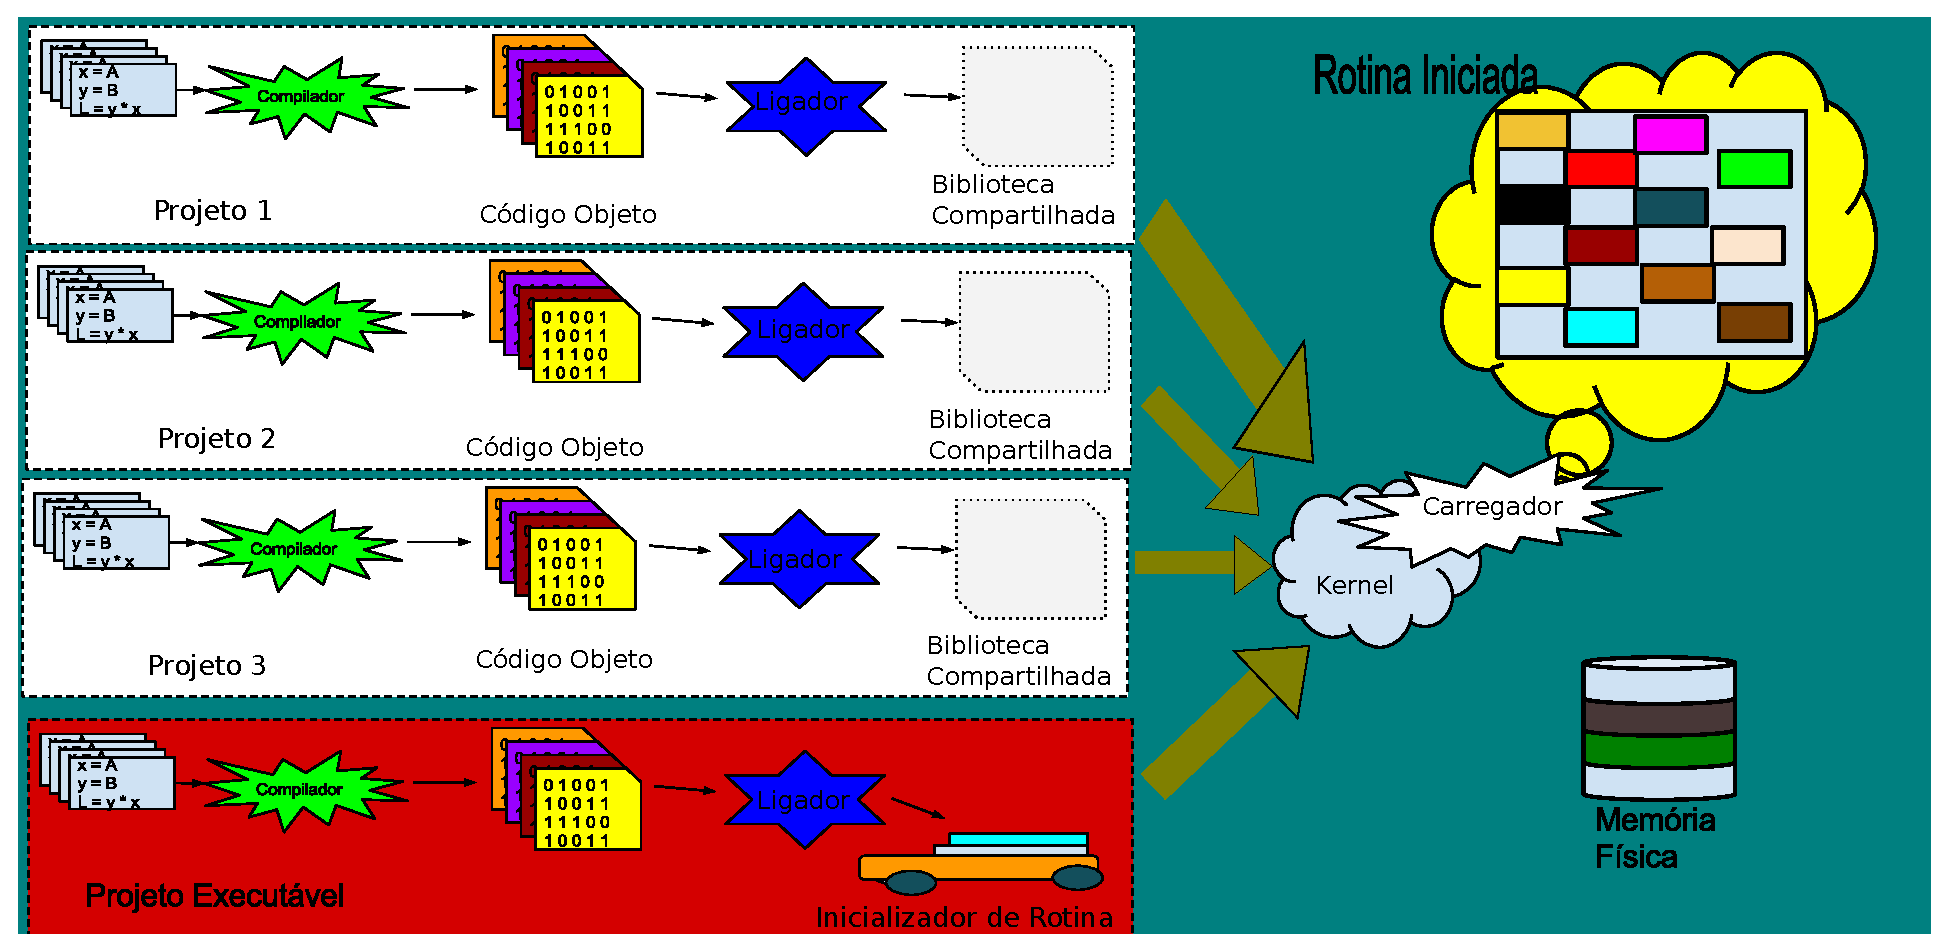
\includegraphics[keepaspectratio=true,scale=0.45]{figuras/dynamic_lib.eps}
    \caption{Biblioteca dinâmica \cite[pág. 55]{ref39}, com adaptações.}
    \label{fig06}
\end{figure}


\section{Métodos para a redução do tempo de compilação}

\subsection{Guardas de Inclusão}\label{include_guards_section}

Em C++, a inclusão de um arquivo de código fonte em outro arquivo fonte é feita
 através da diretiva de pré-processamento chamada \texttt{\#include}, que pode 
ser utilizada como mostrado no Código \ref{codigo_04}. 

\begin{lstlisting}[language=C++,caption={Diretiva de 
                           pré-processamento para inclusão de arquivo},
                                                   label=codigo_04]
// biblioteca de sistema 
#include <nome do arquivo>  

ou

// outras bibliotecas 
#include "nome do arquivo"  

\end{lstlisting}


Diretivas \texttt{\#include} normalmente são utilizadas várias vezes em um projeto.
 No entanto, o preprocessador não é capaz de verificar se um arquivo já foi
 adicionado, o que pode ocasionar um erro de duplicação de definição de
 estruturas e elementos do código. Um exemplo deste problema é mostrado na
 Figura \ref{fig07} \cite[pág. 57]{ref39}.

\begin{figure}[h]
    \centering
        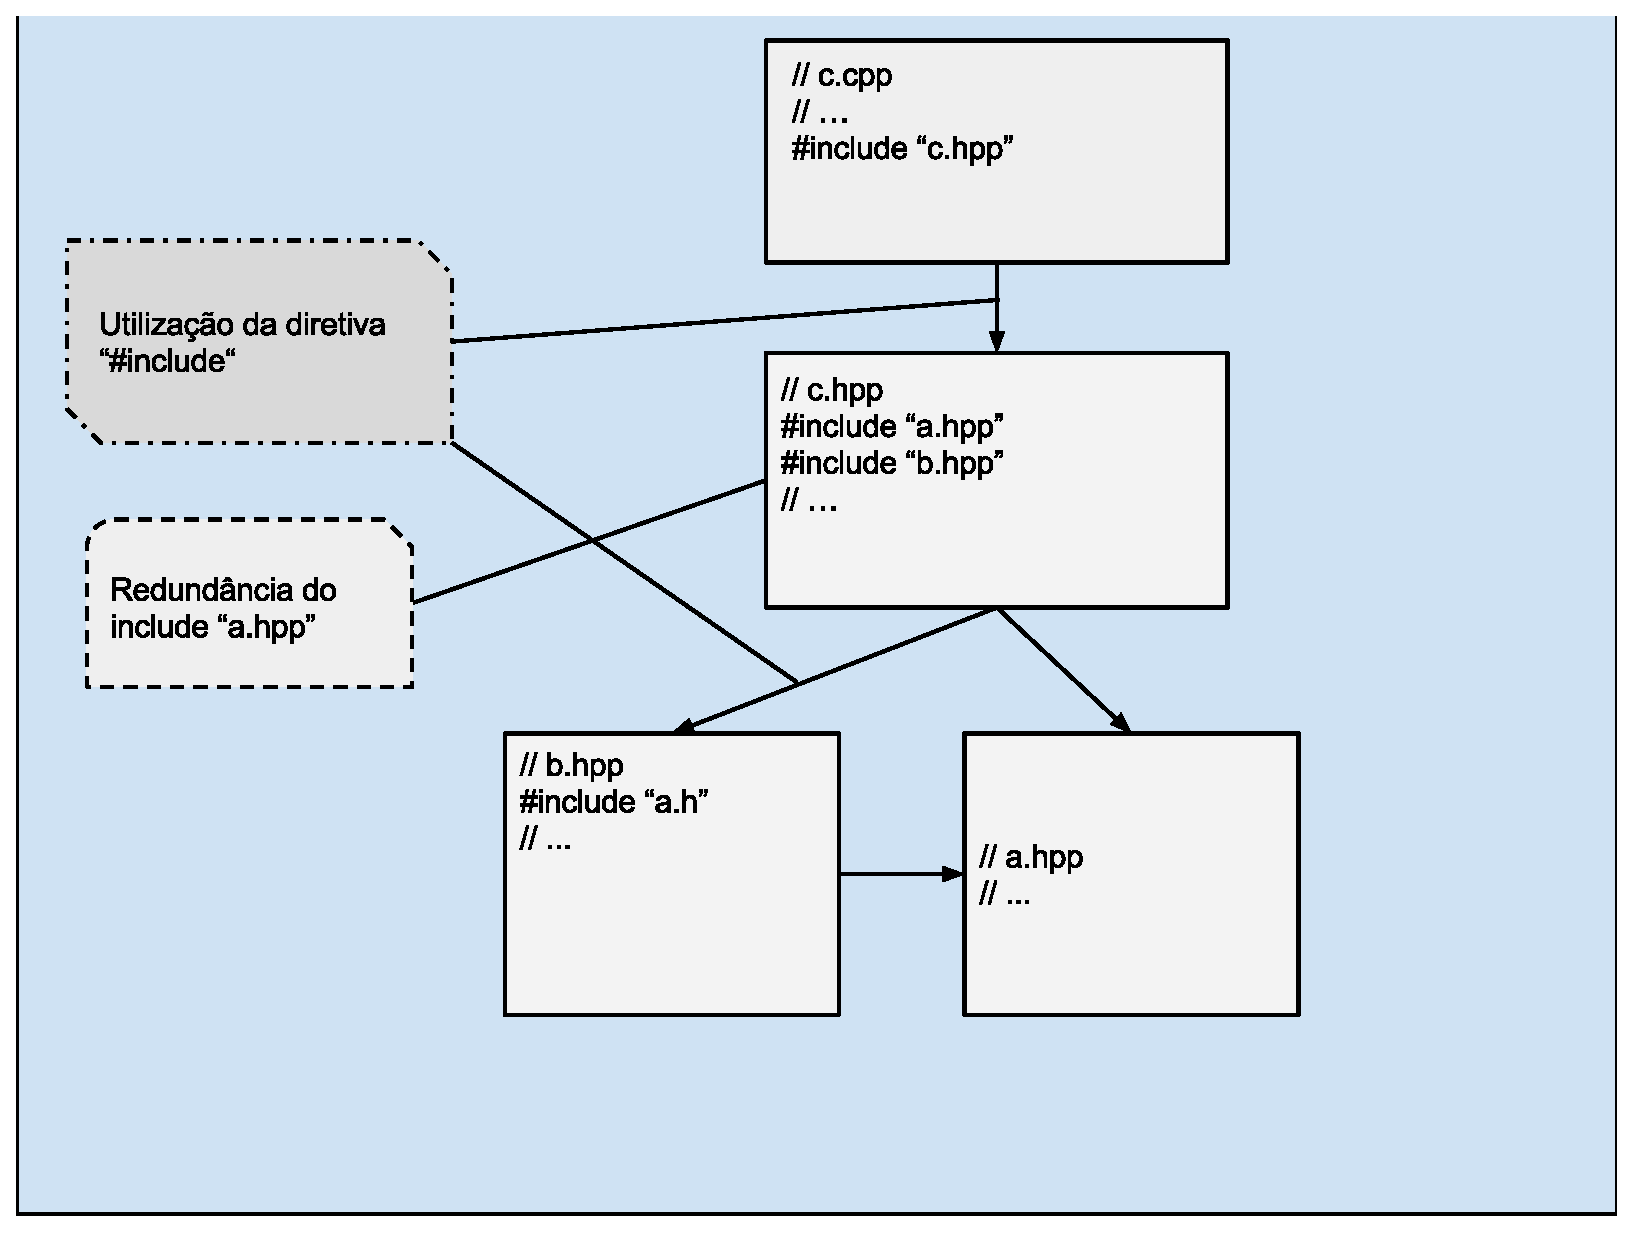
\includegraphics[keepaspectratio=true,scale=0.55]{figuras/multi_include.eps}
    \caption{Includes redundante \cite[pág.  80]{ref42}, com adaptações.}
    \label{fig07}
\end{figure}

Para correção deste problema foram criadas as guardas de inclusão 
(no inglês chamada de  \textit{include guards} ou \textit{guard conditions}),
 que são diretivas de pré-processamento utilizada para verificar se um
 identificador já está definido ou não. Existem varias versões de guardas
 de inclusão, as quais serão citadas adiante \cite[pág. 80]{ref42}.

Normalmente, arquivos-cabeçalho (ou \textit{headers}) são utilizados para
 declarações de estruturas, variáveis, funções e macros. Tais arquivos são
 identificados pelos sufixo \texttt{.h}, \texttt{.hpp}, \texttt{.hxx} ou \texttt{.hpp}. As implementações
 das funções e definições de variáveis são feitas, na maioria das vezes, em
 arquivos denominados fontes (ou \textit{sources}), cujas extensões mais
 comuns são \texttt{.c}, \texttt{.cpp}, \texttt{.cxx}, \texttt{.cc}, \texttt{.c++}, entre outros
 \cite{gccsufix}.

Há quatro tipos de guardas de inclusão:

\begin{enumerate}
\item Interna ao arquivo \textit{header}:

A diretiva \texttt{\#ifndef} é utilizada para verificar se um identificador foi 
 definido (forma negativa, para a forma positiva a diretiva é \texttt{\#ifdef}); a 
diretiva \texttt{\#define} é utilizada para definir um identificador; e a diretiva 
\texttt{\#endif} e utilizada para finalizar  uma condição (diretivas \texttt{\#ifdef} e 
\texttt{\#ifndef}) \cite{ref42}.

Caso o identificador já esteja definido, o preprocessador irá ignorar 
qualquer informação que que esteja entre as diretivas \texttt{\#ifndef}  e \texttt{\#endif};
 caso não esteja definido, o identificador serão então definido e as informações
 que seguem a diretiva serão incluídas no arquivo resultante \cite[pág. 80]{ref42}.

Os Códigos \ref{codigo_004}, \ref{codigo_05} e \ref{codigo_06} ilustram uma 
guarda de inclusão interna ao arquivo \textit{header}.

\begin{lstlisting}[language=C++,caption={
						Arquivo c.hpp contendo guardas de inclusão interna},
                                                            label=codigo_004]
// c.h  declaracao de variavel
// verficar se o simbolo INCLUDE_C esta definido
#ifndef INCLUDE_C   
// define um simbolo INCLUDE_C
#define INCLUDE_C   

#include "a.hpp"      // importa o arquivo "a.hpp"
#include "b.hpp"      // importa o arquivo "b.hpp"

...                 // define as estruturas

#endif              // fim da condicional "#ifndef" 
\end{lstlisting}

\begin{lstlisting}[language=C++,caption={
                                     Arquivo b.hpp que inclue o arquivo a.h},
                                                            label=codigo_05]
// b.hpp
#ifndef INCLUDE_B
#define INCLUDE_B

 #include "a.hpp"

 // declaracao de estruturas 
 ...
#endif    
\end{lstlisting}

\begin{lstlisting}[language=C++,caption={
                        Arquivo a.hpp contendo guardas de inclusão interna},
                                                            label=codigo_06]
// a.hpp    arquivo de declaracao
#ifndef INCLUDE_A
#define INCLUDE_A

  // declaracao de estruturas 
  ...

#endif
\end{lstlisting}


\item Externa ao arquivo de \textit{header}:
 
Na  guarda de condição externa  são utilizadas as mesmas diretivas da interna,
 sendo a única diferença é a localização das diretivas: elas antecederão cada uso
 da diretiva \texttt{\#include}. Um exemplo da utilização de guarda de condição 
externa é mostrado nos Código \ref{codigo_07}, \ref{codigo_08} e
 \ref{codigo_09} \cite[pág. 80]{ref42}.


\begin{lstlisting}[language=C++,caption={
					    Arquivo c.hpp contendo guardas de inclusão externa},
                                                            label=codigo_07]
// c.hpp arquivo de declaracao de estruturas de c

#ifndef INCLUDE_A
#define INCLUDE_A
/* inclue o arquivo a.hpp caso o simbolo 
   INCLUDE_A nao esteja definido */
#include "a.hpp"
#endif
        
#ifndef INCLUDE_B
#define INCLUDE_B
 /* inclue o arquivo b.hpp caso o simbolo 
    INCLUDE_B nao esteja definido */
 #include "b.hpp"
#endif

 ... //implementa as declaracoes

\end{lstlisting}

\begin{lstlisting}[language=C++,caption={
						   Arquivo a.hpp com guarda de inclusão externa},
                                                         label=codigo_08]
// a.hpp         declaracao das estruturas de a.hpp

...

\end{lstlisting}

\begin{lstlisting}[language=C++,caption={
					         Arquivo b.hpp com guarda de inclusão externa},
                                                           label=codigo_09]
//b.hpp        declaracao das estruturas de b.hpp

...

\end{lstlisting}


\item Redundância:\label{redundancia_melhor}

Consiste em utilizar, simultaneamente, as guardas de inclusão internas e 
externas. 

Segundo John Lakos \cite[pág. 82]{ref42}, esta guarda de inclusão é a mais trabalhosa de ser mantida
 mas, no entanto, é a que mais reduz o tempo de compilação de um projeto. Ele
 aplicou a técnica de guardas de inclusão com e sem redundância,
 e obteve os resultados mostrados nas Tabelas \ref{tab:tabela_01} e 
\ref{tab:tabela_02}.

\begin{table}[!ht]
    \centering
    \caption {Amostra de Redundância com 10 \textit{headers} por linha}
    \label{tab:tabela_01}
    \begin{tiny}
    \begin{tabular}{cccc}
    \toprule
    \textbf{Quantidade de Arquivos} & \textbf{Sem Redundância(SR)} & \textbf{Com Redundância(CR)} &  \textbf{SR/CR} \\
    \midrule
    1 		& 0,2 	 segundos	 & 0,2 	 segundos		& 1,0	 segundos   \\
    2 		& 0,2 	 segundos	 & 0,2 	 segundos		& 1,0	 segundos   \\
    4 		& 0,3 	 segundos	 & 0,3 	 segundos		& 1,0	 segundos   \\
    8 		& 0,5	 segundos	 & 0,3 	 segundos		& 1,67	 segundos   \\
    16 		& 0,7 	 segundos	 & 0,4 	 segundos		& 1,75	 segundos   \\
    32 		& 1,5 	 segundos	 & 1,1 	 segundos		& 3,0	 segundos   \\
    64 		& 0,2 	 segundos	 & 0,2 	 segundos		& 1,0	 segundos   \\
    128		& 25,9	 segundos	 & 3,5 	 segundos		& 74,0	 segundos   \\
    256		& 126,5	 segundos	 & 13,6  segundos		& 9,3	 segundos   \\
    512 	& 702,3	 segundos	 & 61,6  segundos		& 11,4	 segundos   \\
    1024	& 4378,5 segundos     & 306, segundos6 		& 14,28	 segundos   \\
    \bottomrule
    \end{tabular}
    \end{tiny}
\end{table}

\begin{table}[!ht]
    \centering
    \caption {Amostra de Redundância com 100 headers por linha }
    \label{tab:tabela_02}
    \begin{tiny}
    \begin{tabular}{cccc}
    \toprule
    \textbf{Quantidade de Arquivos} & \textbf{Sem Redundância(SR)} & \textbf{Com Redundância(CR)} &  \textbf{SR/CR} \\
    \midrule
    1 			& 0,2 	 segundos		& 0,2  segundos		& 1,0		segundos \\
    2 			& 0,2 	 segundos		& 0,2  segundos		& 1,0		segundos \\
    4 			& 0,4 	 segundos		& 0,3  segundos		& 1,33		segundos \\
    8 			& 0,7 	 segundos		& 0,4  segundos		& 1,75		segundos \\
    16 			& 1,7 	 segundos		& 0,5  segundos		& 3,4		segundos \\
    32 			& 5,8 	 segundos		& 0,9  segundos		& 6,44		segundos \\
    64 			& 22,1 	 segundos		& 2,0  segundos		& 11,05		segundos \\
    128 		& 89,5 	 segundos		& 5,2  segundos		& 17,21		segundos \\
    256 		& 376,5  segundos		& 17,1 segundos 	& 22,02		segundos \\
    512 		& 1697,4 segundos 		& 68,6 segundos 	& 24,74		segundos \\
    1024 		& 8303,8 segundos 		& 330,6  segundos 	& 25,12		segundos \\
    \bottomrule
    \end{tabular}
    \end{tiny}
\end{table}

\item \textit{Pragma Once}

\textit{Pragma once} é uma diretiva de pré-processamento que possui o objetivo de
 garantir que um arquivo será lido apenas uma vez: caso uma diretiva 
\texttt{\#include} seja utilizada novamente e o arquivo já foi incluído anteriormente,
 o mesmo não será aberto. No entanto, esta implementação se tornou obsoleta 
 na implementação no gcc \cite{gccpragmaonce}. Os Códigos \ref{codigo_10}, \ref{codigo_11} e \ref{codigo_12} exemplificam o uso desta diretiva.



\begin{lstlisting}[language=C++,caption={
                Arquivo c.hpp com guarda de inclusão \texttt{\#pragma once}},
                                                            label=codigo_10]
// c.hpp
/* pragma once indicar que o 
   arquivo c.hpp sera
   incluido apenas 1 vez */
#pragma once            
#include "a.hpp"
#include "b.hpp"

 // declaracoes de c.hpp

 ...

\end{lstlisting}

\begin{lstlisting}[language=C++,caption={
               Arquivo a.hpp com guarda de inclusão \texttt{\#pragma once}},
                                                            label=codigo_11]
// a.hpp
#pragma once 

 // declaracoes de a.hpp

 ...

\end{lstlisting}

\begin{lstlisting}[language=C++,caption={ 
              Arquivo b.hpp com guarda de inclusão \texttt{ \#pragma once}},
                                                            label=codigo_12]
//b.hpp
#pragma once 

 // declaracoes de b.hpp

 ...

\end{lstlisting}

\end{enumerate}

\subsection{\textit{Forward Declaration}}\label{forward_declaration_section}

Em C++, todas as entidades (variáveis, funções, classes, estruturas, uniões,
 etc) deve sem declaradas ou definidas antes de serem referenciadas. Definir
 uma classe antes dela ser utilizada não é possível quando as duas classes
 diferentes referenciam uma a outra, gerando uma referência cíclica
\cite{ref43}.

Considere um exemplo de duas classes, Doutor e Paciente, apresentadas no 
Código \ref{codigo_13}. Neste exemplo, a classe Doutor requer a 
declaração ou definição da classe Paciente, e a classe Paciente necessita 
de uma declaração ou de uma definição da classe Doutor. Desta forma, a 
compilação geraria um erro, pois antes de utilizar uma referência é 
necessário declarar ou definir esta referência.

\begin{lstlisting}[language=C++,caption={
                        Implementação de classes Paciente e Doutor},
                                                     label=codigo_13]
// doutor_paciente.cpp

class Doutor {

  // implementacoes privadas
  private:

  /* a classe Doutor necessita saber que existe 
     a referencia para a classe Paciente */
  Paciente* p; 

  ...          

  // implementacoes publicas
  public:

  ...	

};

class Paciente {

 // implementacoes privadas
 private:

 /* a classe paciente necessita saber que 
 existe a classe Doutor, no entanto
 doutor so existe se souber da referencia
 de paciente */
 Doutor * d; 

 ...  

 // implementacoes publicas
 public:

 ...  

};

\end{lstlisting}

Para resolver este problema é preciso utilizar uma 
referência incompleta (\textit{forward}) da classe Doutor e da
 classe Paciente, conforme apresentado no Código \ref{codigo_14}. 

\begin{lstlisting}[language=C++,caption={ 
           Implementação de classes utilizando \textit{forward declaration}},
                                                    label=codigo_14]
// forward declaration
class Doutor;   
class Paciente; 

class Doutor   {
  // implementacoes privadas
  private:

  /* a referencia incompleta de Paciente existe,
   entao Doutor pode armazenar a 
   referencia do paciente */

  Paciente* p; 
  
  ... 

  // implementacoes publicas
  public: 

  ...
 
};

class Paciente {
  // implementacoes privadas
  private:
	
  Doutor * d; 

  ... 
	
  // implementacoes publicas
  public: 

  ...

};

\end{lstlisting}

A declaração incompleta (\textit{forward declaration}) de uma classe somente podem
 ser utiliza em arquivos na forma de ponteiro (utilizando o operador \texttt{*})
 ou referência (utilizando o operador \texttt{\&}), pois estas não requerem uma
 definição de classe completa porque, em C++, é alocado uma quantidade fixa
 de memória para estes tipos de variáveis \cite[pág. 111]{ref43}.

Um exemplo incorreto de utilização de \textit{forward declaration} seria utilizar
 um construtor da classe Doutor é mostrado no Código \ref{codigo_15}.


\begin{lstlisting}[language=C++,caption={
                          Uso incorreto de \textit{forward declaration}},
                                                label=codigo_15]
   // forward declaration
   class Doutor;

   // utilizacao da estrutura Doutor
   Doutor doutor();

\end{lstlisting}

Como já mencionado, qualquer entidade deve ser declarada ou definida antes
 de ser utilizada, então o caso acima é válido para funções, variáveis,
 estruturas e uniões, entre outros. A Tabela \ref{tab:tabela_03} mostra
 um exemplo de \textit{forward declaration} para alguns destes tipos
 de estruturas.

\begin{table}[!ht]
    \centering
    \caption{Exemplos de \textit{forward declaration}}
    \label{tab:tabela_03}
    \begin{tabular}{>{\ttfamily}l>{\ttfamily}l}
    \toprule
    \textbf{Definição} & \textbf{Declaração} \\
    \midrule
    int x; & extern int x;\\
    \rowcolor[gray]{0.9}
    typedef struct Foo\{int x;\}; & typedef struct Foo;\\
    class Foo \{ int x;public: Foo() ... \}; & class Foo;\\
    \rowcolor[gray]{0.9}
    int Add(int x ,int  y) \{ return x + y; \} & int Add(int x, int y);\\
    union Foo \{ int x; char x; \} Foo; & union Foo;\\
    \bottomrule
    \end{tabular}
\end{table}


Na linguagem C++ há uma separação entre  a implementação e a interface de
 classe \cite[pág. 140]{ref44}. Na maioria dos casos, a definição de uma classe possui
 detalhes de sua implementação, como nos Código \ref{codigo_16} e \ref{codigo_17}.


\begin{lstlisting}[language=C++,caption={ 
                                 Declaração da classe Pessoa},
                                                label=codigo_16]

// pessoa.hpp   - declaracao da classe
#ifndef PESSOA_HPP
#define PESSOA_HPP

// conhecer detalhes de implementacao da string
#include <string>       
// conhecer detalhes de implementacao da Data
#include "data.hpp"     

class Pessoa{
public:

  Pessoa(std::string nome,Data data);
  std::string meu_nome() const;
  Data meu_aniversario() const;

private:
  // detalhes de implementacao na declaracao
  std::string nome;        

  // detalhes de implementacao na declaracao
  Data aniversario;        
};

#endif

\end{lstlisting}

\begin{lstlisting}[language=C++,caption={
                                        Definição da classe Pessoa},
                                                    label=codigo_17]
// pessoa.cpp implementacao da classe
#include "pessoa.hpp"

Pessoa::Pessoa(std::string nome, Data data)
        : nome(nome),aniversario(data)
{
}

std::string
Pessoa::meu_nome() const
{
        return nome;
}
Data
Pessoa::meu_aniversario() const
{
        return aniversario;
}

\end{lstlisting}    


Definir uma classe com detalhes de implementação em sua definição não é uma
 boa prática de programação, uma vez que ela não pode ser compilada sem
 conhecer as definições das classes utilizadas em sua implementação para
 realizar alocação de memória. Isso conduz à utilização da diretriz
 \texttt{\#include}, gerando dependência entre arquivos \cite[pág. 140]{ref44}.

Uma maneira de contornar este problema é utilizar uma \textit{forward declaration} e a
 armazenar referências das classes, de modo que as definições das classes não
 possuam dependência uma das outras. Isto evita que definições de classes sejam
 modificadas com frequência e reduz a quantidade de recompilações devidas às
 dependência entre os  arquivos. Veja os Códigos \ref{codigo_18} 
e \ref{codigo_19}.


\begin{lstlisting}[language=C++,caption={Arquivo definição da classe Pessoa,       
                          utilizando \textit{forward declaration}},
                                                label=codigo_18]
// pessoa.hpp 
#ifndef PESSOA_HPP
#define PESSOA_HPP

// header para string forward declaration
#include <bits/stringfwd.h>    

// forward declaration
class Data;            

class Pessoa{
public:
        Pessoa(std::string& nome,Data *data);
        std::string& meu_nome() const;
        Data* meu_aniversario() const;

private:
// referencia para string
  std::string& nome;

// referencia para Data
  Data* aniversario;
};

#endif

\end{lstlisting}


\begin{lstlisting}[language=C++,caption={ 
Definição da classe Pessoa, utilizando \textit{forward declaration}},
                                                    label=codigo_19]
// pessoa.cpp -  implementacao
#include "pessoa.hpp"
#include <string>

Pessoa::Pessoa(std::string& nome, Data* data)
        : nome(nome),aniversario(data)
{
}
std::string&
Pessoa::meu_nome() const
{
        return nome;
}
Data*
Pessoa::meu_aniversario() const
{
        return aniversario;
}

\end{lstlisting}


O Código \ref{codigo_18} foi feito o uso da diretiva \texttt{\#include
 <bits/stringfwd.h>}. Em C++  existem arquivos-cabeçalhos que possuem a
 implementação de \textit{forward declaration}. A Tabela \ref{tab:tabela_04} lista 
 alguns \textit{forward declaration} que podem ser utilizados em C++ segundo
 o tipo de biblioteca padrão gcc-gnu \cite{gccapi}.

\begin{table}[h]
    \centering
	\caption {Tabela de Algumas \textit{forward declaration} padrões do C++}
    \label{tab:tabela_04}
	\begin{tabularx}{0.95\textwidth}{>{\ttfamily}l>{\ttfamily}X}
	\toprule
	\textbf{Biblioteca} & \textbf{Alguns includes do header}\\
	\midrule
	\#include <bits/stringfwd.h> & std::string, std::wstring, std::u16string, std::u32string; \\
	\midrule
	\#include <iosfwd>          & std::filebuf, std::fstream, std::ifstream, std::iostream, std::istream, std::ofstream, std::ostream, std::ostringstream, std::stringbuf, std::streambuf, entre outros;\\
	\midrule
	\#include <bits/localefwd.h> & std:has\_facet, std::isalnum, std::isalpha, std::iscntrl, std::isdigit,std::isgraph, std::islower, std::isprint, std::ispunct, std::isspace, std::issuper, entre outros;\\
	\midrule
	\#include <bits/algorithmfwd.h> & std::adjacent\_find, std::any\_of, std::binary\_search, std::copy\_backward, std::copy\_if, std::count\_if, std::count, std::find\_end, std::find\_if, entre outros.\\
	\bottomrule
	\end{tabularx}
\end{table}


\subsection{Makefile}\label{Makefile_section}


Make é uma ferramenta utilizada para determinar automaticamente quais
 trechos de código de um grande projeto precisam serem recompilados
 após alguma iteração de desenvolvimento. Esta ferramenta foi implementada
 por Richard Stallman e Roland McGrath, desde a versão 3.76 até os dias de
 hoje vem sendo mantida por Paul D.Smith \cite{Lasca2}. O manual de utilização do \texttt{makefile}
 é disponibilizado no portal GNU \cite{ref45}.

Para utilizar a ferramenta make é necessário a criação de um arquivo chamado
 \texttt{makefile}, que contém as descrições de relações entre os arquivos em um projeto
 e comandos necessários para realizar as atualizações em cada arquivo \cite{Lasca2}.
 Depois de definir o arquivo \texttt{make}, utiliza a chamada de sistema apresentada 
no Código \ref{codigo_20}.

\begin{lstlisting}[language=C++,caption={
                             Chamada de sistema para executar o programa make},
				                                                label=codigo_20]
    $ make
\end{lstlisting}


O programa make realiza as devidas verificações nos códigos fontes e
 nos artefatos, e caso seja necessário recompilar um arquivo, o
 \texttt{makefile} contém as instruções necessárias para o tal procedimento
 \cite[pág. 1]{ref45}.


\subsection{Estrutura básica de um arquivo \texttt{makefile}}

Arquivos \texttt{makefile} contém 5 tipos básicos de elementos: regras explicitas,
 regras implícitas, definição de variáveis, diretivas e comentários.

\begin{enumerate}

    \item Regras Explicitas: \
        conjunto de regras que informam quando e como refazer as construções
         de arquivos. Ela é definida pela estrutura apresentada no Código \ref{codigo_21}.


        \begin{lstlisting}[language=C++,caption={
                                     			Regras explicitas de Makefile},
                                                        label=codigo_21]

alvo ... : pre-requisitos ... 
    procedimentos
	...
ou 

alvo ... : pre-requisitos ... ; procedimentos
    procedimentos
    ...

        \end{lstlisting}


 O \textbf{alvo} é utilizado para nomear os artefatos que devem ser gerados pelo projeto.
 O alvo também pode ser utilizado para fazer a chamada de execução de um trecho
 específico do Makefile,  sendo passando como parâmetro na utilização do comando
 make.

 Os \textbf{pré-requisitos} são os endereços de arquivos utilizados como entrada para a 
criação do alvo. Este campo é opcional, pois podem existir instruções que não
 necessitam de arquivos de entrada, como por exemplo a instrução \texttt{clean}
 (tipicamente utilizada para remoção de todos os códigos objetos gerados a partir
 dos códigos do projeto) \cite[pág. 1]{ref45}.

Os \textbf{procedimentos} são as ações que devem ser executadas a partir do comando make.
Este bloco pode conter mais de um comando em uma linha, ou  vários comandos em
 linhas separadas \cite[pág. 1]{ref45}.

    \item Regras Implícitas: \
 conjunto de regras que informam quando e como refazer uma classe de arquivos
 baseadas em seus nomes e padrões \cite[pág. 11]{ref45}. Um exemplo de utilização de 
 padrões é apresentado no Código \ref{codigo_22}. \\ \cite[pág. 19]{ref45}
        
    \begin{lstlisting}[language=C++,caption={ 
                                     Utilização de padrões no \texttt{makefile}},
                                                        label=codigo_22]

# gerar  objetos .o utilizando arquivos .c
%.o : %.c
    procedimentos
    ...

    \end{lstlisting}


    \item Definição de Variáveis:\
 é uma linha que especifica um valor para uma variável que pode ser substituída no
 texto posteriormente \cite[pág. 111]{ref43}. Veja o Código \ref{codigo_23} para um exemplo de 
definição de variável.

    \begin{lstlisting}[language=C++,caption={ 
                                     Definição e utilização de variável},
                                                         label=codigo_23]
objetos = main.o command.o display.o files.o search.o utils.o

clean:
    rm $(objetos)
    \end{lstlisting}


    \item Diretivas: \
são instruções que indicam ao make ações especiais a medida que é realizada a leitura do
 arquivo Makefile \cite[pág. 22]{ref45}. Estas instruções podem ser:

    \begin{itemize}
        \item Realizar a leitura de um outro \texttt{makefile}, através da diretiva include, seguida do nome do arquivo.
        \item Utilizar ou ignorar parte do \texttt{makefile} \cite[pág. 22]{ref43}. O Código \ref{codigo_24} ilustra o uso desta diretiva. 


    \begin{lstlisting}[language=C++,caption={ 
                                      Makefile com diretiva condicional},
                                                         label=codigo_24]

ibs_for_gcc = -lgnu
normal_libs =

foo: $(objects)
ifeq ($(CC),gcc)
$(CC) -o foo $(objects) $(libs_for_gcc)
else
$(CC) -o foo $(objects) $(normal_libs)
endif

    \end{lstlisting}

    \begin{itemize}
        \item \textbf{ifeq:} Diretiva que começa a condicional e especifica a 
    condição. Ela contém 2 argumentos, separados por virgula e entre parêntesis.
     Caso os argumentos forem iguais as linhas entre o \textbf{ifeq} e o
     \textbf{else} serão executadas, caso contrário serão ignoradas \cite[pág. 77]{ref45}.

        \item \textbf{else:} Diretiva que marca o início das instruções a serem 
    executadas caso a condição do \textbf{ifeq} falhe. Esta diretiva é opcional \cite[pág. 77]{ref45}.

        \item \textbf{endif:} Diretiva que finaliza a condição. 
    Toda diretiva condicional condição deve ser terminada com endif \cite[pág. 77]{ref45}.
    \end{itemize}

    \item Definir variáveis com mais de uma linha. Com a utilização da diretiva \textit{\#define}
 e  da diretiva \textit{\#endif} é possível realizar a definição de uma variável em mais
 de uma linha \cite[pág. 69]{ref45}. O Código \ref{codigo_25} ilustra esta situação.

    \begin{lstlisting}[language=C++,caption={
			 	Makefile com definição de variável em múltiplas linhas},
														label=codigo_25]
bar= "BAR"
define two-lines =
echo foo
echo $(bar)
endef
all:
$(two-lines)
    
    \end{lstlisting}


    \end{itemize}

    \item Comentários: \
Em arquivos Makefile a utilização de caractere \texttt{\#} em uma linha faz com
 que todos o caracteres que o sucederem sejam ignorados. Caso seja necessário
 a utilização deste caractere basta precedê-lo com o caractere \texttt{\textbackslash} (barra invertida) \cite{ref45}.

\end{enumerate}


\subsection{Padrões de um arquivo \texttt{makefile} para ferramentas GNU}

    
Tendo como referência o manual do GNU Make\footnote{
\url{http://www.gnu.org/software/make/manual/make.pdf}},
Seção 15.6, existem padrões que podem ser utilizados em arquivo
 \texttt{makefile}. Alguns dos mais comuns são:

\begin{enumerate}
    \item \textbf{all}: instrução executada por default pelo \texttt{makefile}, 
realiza as verificações do arquivos de código fonte e faz atualizações
 nos códigos objetos, se necessário;
    \item \textbf{install}: chama o make all e copia os arquivos 
executáveis, bibliotecas, e os demais artefatos do projeto para os 
locais adequados, de acordo com as necessidades do projeto;
    \item \textbf{uninstall}: deleta todos os arquivos copiados 
pelo comando make install;
    \item \textbf{clean}: deleta todos os arquivos e diretórios 
criados na construção do programa final;
    \item \textbf{distclean}: remover os arquivos que foram gerados
 por algum comando make, seja na configuração, seja na
 construção de um programa;
    \item \textbf{info}: gera um arquivo de informações sobre o programa;
    \item \textbf{dist}: gera um arquivo \texttt{tar} cujo nome contém a versão e
o nome do projeto e  que inclui  todo o conteúdo do diretório atual;
    \item \textbf{check}: gera o programa  e realiza testes;
    \item \textbf{installcheck}: gera o programa, instala e realiza testes;
    \item \textbf{installdirs}: cria  os diretórios onde os arquivos devem ser instalados.
\end{enumerate}


\subsection{Executando o \texttt{make}}

Depois de gerado o arquivo \texttt{makefile} utilizando as regras descritas nas seções anteriores,
 o comando \texttt{make} pode ser utilizado para executar as regras descritas.
O comando pode ser utilizado como mostrado no Código \ref{codigo_26} e conforme apresentado na Tabela \ref{tab:tabela_05},


    \begin{lstlisting}[language=C++,caption={ 
                                             Utilizando o programa make},
                                                         label=codigo_26]
        $ make [opcoes] ... [Alvo]

    \end{lstlisting}


onde \textbf{alvo} é a instrução que será executada pelo \textit{make}(A omissão deste
parâmetro leva a execução do alvo \textit{all}) e \textbf{opções} são flags de controle
 utilizadas pelo utilitário make. Exemplos de flags estão definidas na Tabela \ref{tab:tabela_05}:

\begin{table}[h]
    \centering
    \caption {Exemplos de flags que podem ser utilizadas no make}
    \label{tab:tabela_05}
    \begin{tabular}{ lp{8cm}}
    \toprule
    \textbf{Flag} & \textbf{Descrição}\\
    \midrule
    \texttt{-C dir} , \texttt{--directory=dir} & Modifica o diretório antes de fazer a leitura do \texttt{makefile}\\
    \midrule
    \texttt{-f file}, \texttt{--file=file}, \texttt{--makefile=FILE} & Realiza a leitura de um \texttt{makefile} especifico\\
    \midrule
    \texttt{-i}, \texttt{--ignore-errors} & Ignora erros na reconstrução de arquivos\\
    \midrule
    \texttt{-I dir}, \texttt{ --include-dir=dir} & Especifica o diretório que inclue os \texttt{makefiles}\\
    \midrule
    \texttt{-j [jobs]}, \texttt{--jobs[=jobs]} & Especifica a quantidade de threads
                                 que podem ser executadas em paralelo. 
                                 Caso não seja passado a quantidade de
                                 threads ele não terá limites na criação
                                 de threads.\\
    \bottomrule
    \end{tabular}
\end{table}


\subsection{\textit{Pimpl Idiom} - Implementação privada} \label{Pimpl_Idiom}

Ponteiro de implementação é a técnica utilizada para armazenar a
 implementação privada de uma estrutura em um ponteiro, que será
 declarado nos arquivos de \textit{header} e implementado nos arquivos de
 implementação, através da utilização da declaração incompleta 
 (\textit{Forward Declaration}).

Esta técnica, ao ser utilizada, tem como benefício minimizar a
 interdependência entre estruturas e, por consequência, diminui o
 tempo de recompilação, além de esconder partes que não deveriam
 ser mostradas na declaração de uma classe, pois estas
 deveriam ser privadas \cite{style_idioms}. O Código \ref{exemplo_implementacao_pimpl}
 ilustra esta técnica;

\begin{lstlisting}[language=C++, caption={Exemplo Utilização Pimpl Idiom},
                  label=exemplo_implementacao_pimpl]
    // book.h
    #ifndef  BOOK_H
    #define BOOK_H

    #include <iostream>
    using namespace std;

    class Book
    {
    public:
      Book(string name);
      void read();
    private:
      class BookImpl;        
      BookImpl* m_impl;        
    };
    #endif

    //book.cpp
    class Book::BookImpl
    {
    public:
      BookImpl(string name,int paginas=0,read=false);
      string get_name();
    private:
      string name;
      int paginas;
      bool read;
    };



    Book::BookImpl::BookImpl(string name,int paginas,bool read)
      : name(name), paginas(paginas),read(read)
    {
    }


    Book::BookImpl::string get_name()
    {
        return this->name;
    }

    Book::Book(string name)
      : m_impl(new BookImpl(name))
    {
    }

    void
    Book::read()
    {
      cout << this->m_impl->get_name() <<endl;
    }

    //main.cpp
    #include <iostream>
    #include "book.h"
    using namespace std;
    int main()
    {
      Book a("eBook");
      a.read();
      return 0;
    }
\end{lstlisting}

\subsection{Flags de Otimização de Baixo Nível}
\label{Otimizacao_de_baixo_nivel}

Como visto na Seção \ref{Compilação} é possível otimizar
 o código para gerar objetos e executável menores e com tempo de
 execução mais rápida, no entanto ao executar este processo, o compilador perde
 tempo nestas otimizações de modo que o tempo de compilação aumenta.
 Para controlar estas otimizações, os compiladores recebem como \textit{flags} (parâmetros) que
 indicam quais tipos de otimização pode ser aplicadas pelo compilador.\footnote{\url{https://gcc.gnu.org}}

No gcc/g++
\footnote{\url{https://gcc.gnu.org/onlinedocs/gcc/Optimize-Options.html}}
\footnote{\url{https://gcc.gnu.org/onlinedocs/gnat\_ugn/Optimization-Levels.html\#Optimization-Levels}},
 as flags de otimizações de compilação podem ser:

\begin{itemize}
	\item -O0 : reduz o tempo de compilação e faz a depuração produzir os
 resultados esperados. Este é o padrão caso nenhuma \textit{flag} seja passada;
    \item -Ofast : descarta estritas conformidades com padrões;
    \item -O  : realiza otimização do tamanho do código e do tempo de execução do programa.
No entanto não realiza otimizações que tenham grandes perdas no tempo de compilação;
    \item -O1 :  aplica uma otimização moderada, mas não degrada significativamente
 o tempo de compilação;
    \item -O2 : realiza otimização total, gerando o código altamente otimizado e com o
 tempo mais lento de compilação;
    \item -O3 : aplica otimização total como o -O2 , no entanto liga mais flags;
    \item -Os : aplica as otimizações de -O2 que não implicam no aumento do tamanho do código,
 e também otimizações adicionais para a redução do tamanho do código;
    \item -Og : realiza otimizações  que não interferem da depuração,
 oferecendo um nível de otimização razoável e  mantendo a compilação rápida.
\end{itemize}

Caso seja utilizado mais de uma \textit{flag} de otimização, a última passada que será executada
 e as outras serão desconsideradas.


\subsection{Ferramentas}  \label{ferramentas_de_otimizacao}

\begin{itemize}
	\item \textbf{Ccache} \label{ccache}
	
	\subitem Ccache\footnote{\url{https://ccache.samba.org/download.html}} é uma ferramenta utilizada
 para armazenar compilações anteriores e 
guarda os resultados, detectando quando os mesmos serão necessários
 para reduzir o retrabalho do processo de compilação.

    \subitem Esta ferramenta tem suporte às linguagens C, C++, Objective-C and Objective-C++.
Possui as vantagens : gerencia o tamanho de \textit{cache},
 armazena compilações que contém avisos (\textit{warnings}), baixa sobrecarga,
 opcionalmente utiliza “\textit{hard link}” para evitar cópias e comprime arquivos para
 reduzir o tamanho de uso do disco. Apesar de suas vantagens, esta ferramenta pode apenas
 compilar um único arquivo ou link simbólico, funciona somente com compiladores gcc/g++
 ou similares e algumas \textit{flags} de otimização não são suportadas.

	\subitem Para utilizar o \textit{ccache} é necessário adicionar a palavra \textit{ccache} antes de cada
 comando de compilação. Para remover cache de compilação anterior será utilizado
 ccache -c ativar o limpador de ccache e ccache -C para remover a cache completamente.

	\item \textbf{Gold} \label{Gold}

	\subitem Gold é uma ferramenta de linkagem de objetos mais rápida que o linkador padrão do Linux o
 ld. Esta ferramenta foi desenvolvida apenas para realizar linkagem de arquivos do tipo ELF sem utilizar
 a biblioteca BFD (\textit{Binary File Descriptor library}) que possui suporte a manipulação de vários
 formatos de arquivos binários, pelo pesquisador da Google,
 Ian Lance Taylor, que realizou a remoção da biblioteca e utilização de menos camadas de abstrações.

	\subitem O linker \textit{gold} vem por padrão nos pacotes do GNU e pode ser utilizado no gcc/g++ passando a flag
 -Wl,-fuse-ld=gold\footnote{\url{https://gcc.gnu.org/onlinedocs/gcc/Link-Options.html}},
 caso nenhuma \textit{flag} seja passada, será utilizado o linker padrão \textit{ld} que utiliza
 a biblioteca BFD. O linker \textit{gold} para ser utilizado em sistemas com \textit{back-end llvm} é necessário
 instalar o plugin \textit{llvm-gold-plugin}\footnote{\url{http://llvm.org/docs/GoldPlugin.html}}.

	\subitem Para sistemas operacionais como um Mac OS e Windows esta ferramenta não é suportada, uma vez que
estes sistemas possuem formato de arquivo binário diferente do ELF. Windows possui os sistemas de arquivo PE ou PE32+, enquanto o Mac OS utiliza PEF ou XCOFF
\footnote{\url{https://en.wikipedia.org/wiki/Comparison\_of\_executable\_file\_formats\#cite\_note-apple-pef-9}}.
\end{itemize}
